% Part 1: Detecting DNA-bound RecB molecules
\section*{Results}

\subsection*{Imaging DNA-bound RecB molecules}

\begin{figure*}[htbp]
\begin{center}
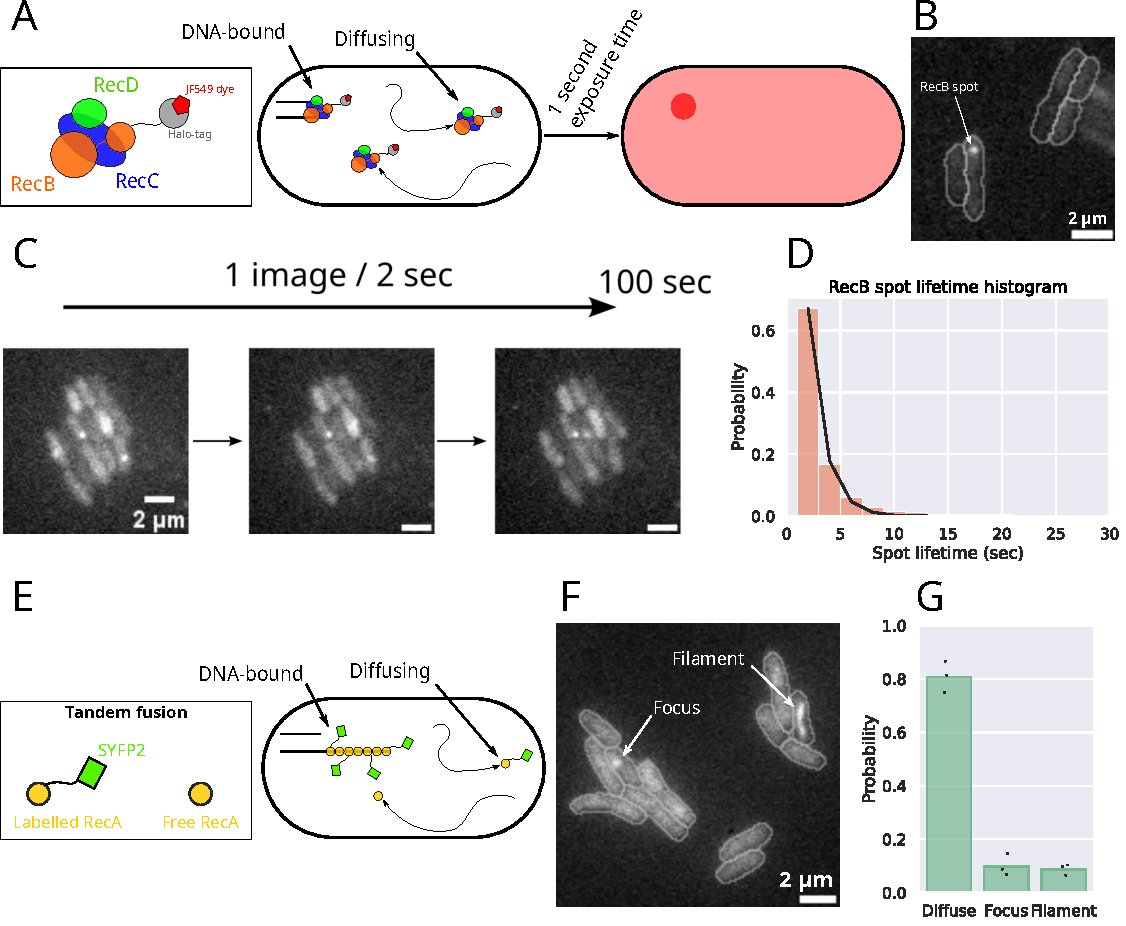
\includegraphics[width=\textwidth]{Fig1_endogenous.pdf}
\end{center}
\caption{Probing DSB repair by RecBCD in live \textit{E. coli}. (A) Scheme of our experimental protocol. The RecB subunit of the RecBCD complex is fused to a Halo-tag, bound by the JF549 fluorescent dye. A long exposure time (1 sec) makes diffusing molecules appear as diffuse signal in the cell, while DNA-bound molecules are visible as bright, diffraction-limited spots. (B) Example image of a RecB spot (white arrow). (C) Example images of a timelapse acquisition (1 image every 2 sec for 100 sec). (D) Histogram of the lifetime of RecB spots (E) Example image of RecA imaging under endogenous DNA damage. RecA is diffuse in most cells, a RecA focus and a RecA filament are visible in two of the cells (white arrows). (F) Proportions of cells containing the different RecA structures (dots: individual datasets, bars: average between datasets).}
\label{Fig:endogenous}
\end{figure*}

%% Explain what we are trying to do (detect RecB binding to DNA)
%% Mention that bacteria experience endogenous damage
%% Explain the experiment principle, conclude with the fact that we are detecting RecB spots (SI control: no spots on the free Halo images)
To image RecBCD in live \textit{E. coli}, we used a Halo-tag fusion to the RecB subunit, conjugated to the JF549 fluorescent dye (Figure \ref{Fig:endogenous}A). The fusion was previously used and characterised in the lab, ensuring specific one-to-one labelling of RecB molecules without adverse effects on the DNA repair process.\cite{Lepore2019} To detect the binding of RecB to DNA, we applied the previously developed technique of XXX (check name in Elf article).\cite{Elf2007}  Since RecB is present at low copy numbers in \textit{E. coli} ($\sim$5 molecules per cell on average\cite{Lepore2019}), imaging live cells with a long exposure time (1 second) made diffusing molecules appear as weak homogeneous signal in the cell, while DNA-bound molecules formed intense diffraction-limited spots (referred to throughout this article as RecB spots). (Figures \ref{Fig:endogenous}A, B) The complete absence of similar spots in cells expressing the free Halo-tag from a plasmid confirmed that these structures were specific to RecB (Supp. Fig. \ref{SIFig:freehalo_image}). Seeing RecB spots in cells that were not exposed to an exogenous source of DNA damage was unsurprising, as these cells are still subject to occasional endogenous DNA damage. This can be due for example to collisions between the replication fork and DNA-bound proteins, and was previously reported to affect $\sim$20\% of cells per cell cycle. (ref Leach)

Acquiring short timelapse videos (50 images over 100 seconds, Figure \ref{Fig:endogenous}C) allowed us to measure the binding time of RecB on DNA (Figure \ref{Fig:endogenous}D). The average lifetime of RecB spots in our experiment was 4.4 s $\pm$ 0.29. This prolonged imaging of the RecB-Halo fusion and quantification of DNA binding times was only possible thanks to the exceptional photostability of the JF549 dye, which displayed slow photobleaching and no blinking (Supp. Note \ref{note:dye_bleaching} and Supp. Fig. \ref{SIFig:dye_bleaching}). 

%% RecA makes foci and filaments
\subsubsection*{RecA occasionally forms foci and filaments}
One of RecBCD's purposes when processing a DSB is to facilitate the loading of the RecA protein on single-stranded DNA. To broaden our view of the repair process downstream of RecBCD, we imaged a tandem fusion of RecA with the fluorescent protein SYFP2.\cite{} Based on the fluorescence distribution in the cells, we identified three states of RecA: diffuse, forming a bright focus, or forming an elongated filament. (Figure \ref{Fig:endogenous}E) Because of the large diversity of shapes observed, especially for RecA filaments, the detection of RecA structures by rule-based algorithms was challenging. Therefore, we designed and trained a deep-learning algorithm capable of classifying individual cells based on the three types of structures cited above. (see Methods and Supp. Figure \ref{SIFig:objectClassifier}) This allowed us to quantify the fraction of cells where RecA is freely diffusing to 81\% $\pm$ 6, RecA foci to 10\% $\pm$ 4, and RecA filaments to 9\% $\pm$ 2 (Figure \ref{Fig:endogenous}F). This is consistent with a minority of cells experiencing DNA damage, and being engaged in the repair process.


% Part 2: Separating genuine RecB binding events
\subsection*{Separating genuine DNA binding events from spurious spots}

\begin{figure*}[htbp]
\begin{center}
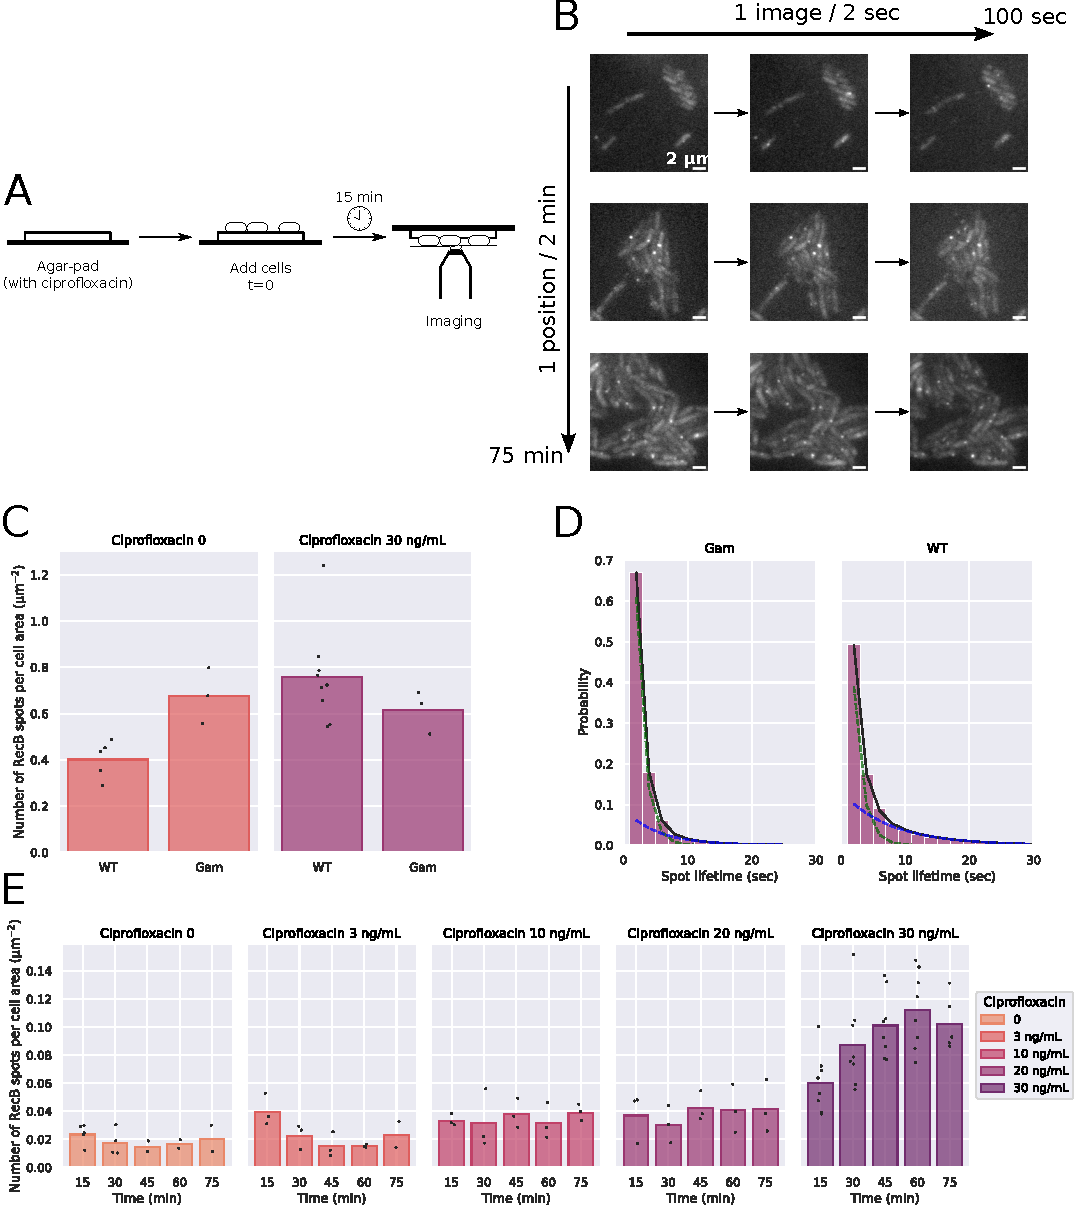
\includegraphics[width=\textwidth]{Fig2_cipro_nSpots.pdf}
\end{center}
\caption{RecB DNA binding under ciprofloxacin exposure. (A) Scheme of cell exposure to ciprofloxacin. The cells are added to a ciprofloxacin-containing agar-pad, and left to settle for 15 min before imaging. (B) Example images of RecB throughout an acquisition. A short timelapse (100 sec) is acquired at a different position every 2 min for 75 min. (C) Number of RecB spots per cell area, at 0 and 30 ng/mL ciprofloxacin (panels) in cells expressing the Gam protein, or not (WT) (D) RecB spot lifetime histograms at 30 ng/mL ciprofloxacin, fitted with a bi-exponential decay model (black line, fit components showed as dashed lines). (E) Number of RecB spots per cell area, as a function of ciprofloxacin concentration (panels) and exposure time to the antibiotic (X-axis). Black dots represent measurements from individual datasets, and solid bars are the average between them.}
\label{Fig:nspots}
\end{figure*}

%% Short description of how ciprofloxacin is added, and the 2 time dimensions
To gain more insight into DNA binding by RecB, we induced additional DSBs by adding ciprofloxacin to agar pads before imaging (Figure \ref{Fig:nspots}A). Cells were left to settle down on the pad for 15 min, and then 50-frame timelapse videos were acquired at a rate of one position every 2 min (Figure \ref{Fig:nspots}B) for 60 min. This allowed us to quantify RecB binding at different time points ranging from 15 to 75 min after ciprofloxacin exposure.

%% Introduce Gam (prevents RecB binding to DNA, etc)
%% Cipro 0: most detected spots are not DNA-binding events
%% Cipro 30: the fact there are less spots in the presence of Gam indicates we are detecting some true DNA binding events
Before drawing any conclusions on RecB binding to DNA, we needed to ensure that the fluorescent RecB spots were indeed the result of RecB binding to the DNA. To do this, we expressed the Gam protein from a plasmid. Gam is a phage protein that associates strongly with the RecBCD complex and prevents its binding to DNA. A reasonable expectation would be that in the presence of Gam, no or very few RecB spots would be observed. In contrast to this, in the absence of ciprofloxacin cells that expressed Gam had more RecB spots per cell area than wild-type cells (Figure \ref{Fig:nspots}C). This shows that unexpectedly, most or all RecB spots observed in the absence of ciprofloxacin are not DNA binding events. We speculate further on the nature of these spurious RecB spots and the reasons behind their increase in the presence of Gam in the Discussion section.
Under exposure to 30 ng/mL ciprofloxacin, we observed an opposite trend, where cells that expressed Gam contained fewer RecB spots than wild-type cells. This confirms that part of the RecB spots (albeit a relatively small fraction) detected under ciprofloxacin exposure do correspond to DNA-bound RecB molecules.

%% Mono-exp fits (SI) show that Gam is ok-fitted by a single population, but WT + cipro is not
%% Bi-exponential fits allow us to separate the spurious spot detections and the genuine DNA binding events
Concomitantly, the lifetime histograms of RecB spots displayed clear differences in the presence and absence of Gam, when DNA damage was induced with 30 ng/mL ciprofloxacin (Figure \ref{Fig:nspots}D and Supp. Figure \ref{SIFig:monoexp_fits}). The difference in the distribution was particularly visible when fitting with a mono-exponential decay function ($y=a.e^{-k.t}$, Supp. Figure \ref{SIFig:monoexp_fits}). Whereas the spot lifetime distribution in the presence of Gam was well-approximated, suggesting a single, homogenous population of spots, the distribution in the wild-type cells was less well-fitted. In particular, the fit did not account for a population of longer-lived RecB spots (over 10 seconds). This suggests that the population of RecB spots that represent true DNA binding events (as seen in Figure \ref{Fig:nspots}D) have longer lifetimes than spurious RecB spots.

%% Using the fits to define a lifetime threshold (16 sec = 99% DNA binding)
%% Counting DNA binding events
To specifically analyse RecB binding to DNA, we used the lifetime histogram fits to define a threshold (16 seconds) above which 99\% of RecB spots are predicted to be DNA binding events. Applying this threshold on our data allowed us to count the number of RecB binding to DNA per cell area at different ciprofloxacin concentrations (Figure \ref{Fig:nspots}E). The average number of RecB spots per cell area increased with ciprofloxacin concentration and duration of exposure, which is consistent with ciprofloxacin creating more DSBs, and hence more substrates for RecBCD binding.


% Part 3: The proportion of long-lived spots increases with ciprofloxacin concentration
\subsection*{Short-lived DNA-bound RecB are engaged in DNA repair}

\begin{figure}[htbp]
\centering
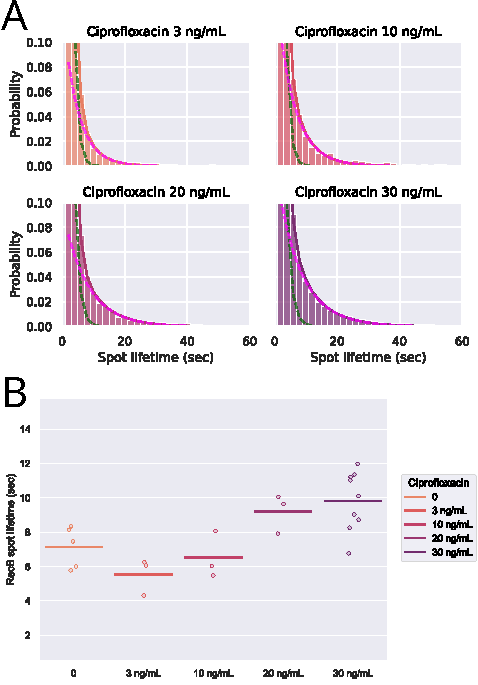
\includegraphics[width=.9\linewidth]{Fig3_cipro_lifetimes.pdf}
\caption{(A) RecB spot lifetime histograms (solid bars) for four different ciprofloxacin concentrations (3, 10, 20 and 30 ng/mL), fitted with a bi-exponential decay model. The top of the histograms was cropped to show the long-lived RecB spots (> 16 sec) more clearly.}
\label{Fig:lifetimes}
\end{figure}


%% RecB spot lifetime histograms are still well fit by two populations
We computed the lifetime histogram of RecB spots at different ciprofloxacin concentrations (3, 10, 20 and 30 ng/mL), and found that all histograms were well-fitted by a model accounting for two populations of RecB spots (Figure \ref{Fig:lifetimes}A). From these fits we retrieved the average binding time of RecB on DNA (Figure \ref{Fig:lifetimes}B). In all conditions, the lifetime was on the order of several seconds, which is in line with RecBCD digesting several kilobases of DNA at a rate of $\sim$1.5 kb/s, as previously reported (ref Cees Dekker?\cite{}). In cells that were experiencing ciprofloxacin damage, the binding time increased from 6 sec $\pm$ 1 to 10 sec $\pm$ 2, which we can tentatively attribute to more challenging DNA repair at higher ciprofloxacin concentrations.

To assess whether the fitted RecB binding times were influenced by our sampling rate (0.5 Hz), we performed control experiments at slower (0.25 Hz) and faster (1 Hz) sampling rates, in the presence of 30 ng/mL ciprofloxacin. These experiments revealed that our initial estimate for the binding time (10 sec $\pm$ 2) is likely to be slightly underestimated (see Supp. note \ref{note:frame_intervals}).



% Part 4: There are two regimes of DNA repair for ciprofloxacin-induced damage
\subsection*{There are two regimes of DNA repair for ciprofloxacin-induced damage}

\begin{figure*}[htbp]
\begin{center}
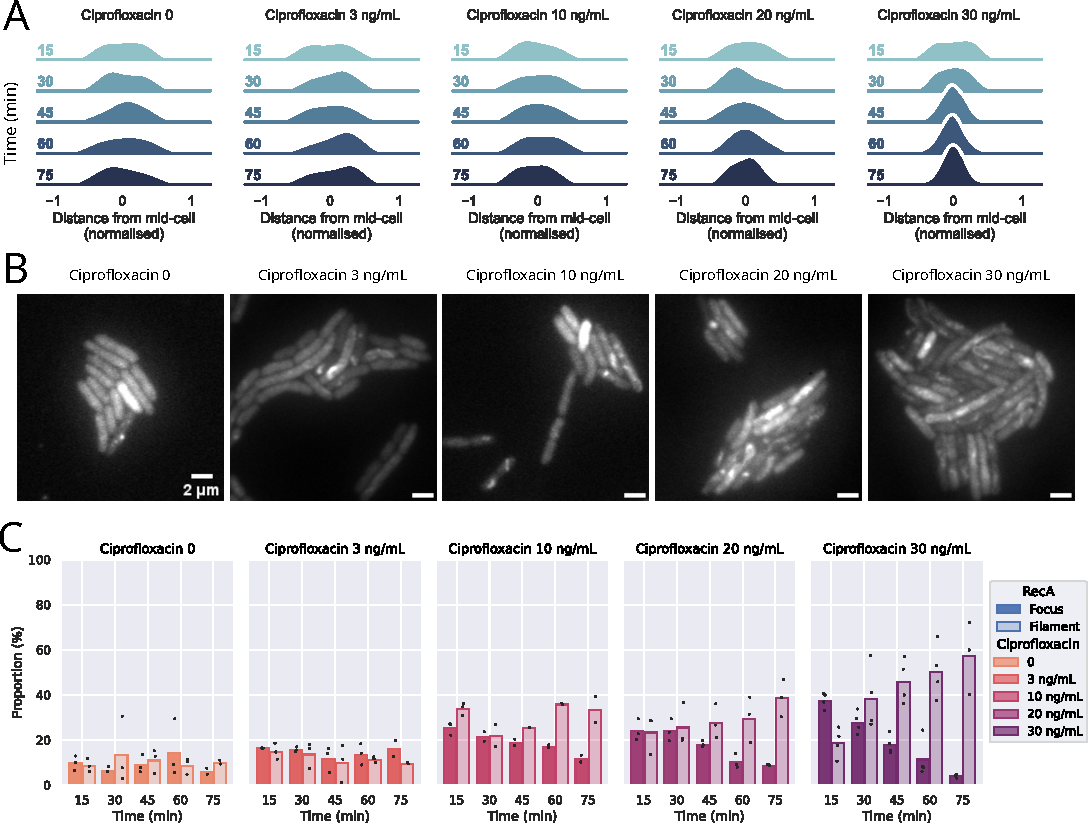
\includegraphics[width=\textwidth]{Fig4_cipro_30ngmL.pdf}
\end{center}
\caption{}
\label{Fig:high_cipro}
\end{figure*}


%% At high cipro (above MIC, 20-30 ng/mL) we see a strong accumulation of RecB spots in the cell (add panel or SI Fig with proportion of cells that have a spot)
%% Moreover these spots are centred in the cell (consistent with SOS/RecN-induced chromosome compaction)
Upon exposure to the higher ciprofloxacin concentrations (20 and 30 ng/mL), the proportion of cells that contain at least one RecB spot increased (Supp. Figure \ref{SIFig:cells_1spot}). This hints at an accumulation of repair intermediates in cells that are exposed to large amounts of DNA damage. Furthermore, whereas at low ciprofloxacin concentrations (0, 3, 10 ng/mL) RecB spots were found throughout the cell, at higher concentrations they appeared more centred in the cell (Figure \ref{Fig:high_cipro}A). This is consistent with RecN-dependent, SOS-induced compaction of the bacterial chromosome upon DNA damage, as has been previously reported (cite RecN paper).

%% We also see a strong accumulation of RecA filaments (RecA foci seem to be transient and their number decreases over time)
Simultaneously with the increase in the number of RecB spots, RecA filaments became visible in a large number of cells (Figure \ref{Fig:high_cipro}B). After one hour of exposure to ciprofloxacin, the proportion of cells that contained a RecA filament was $\sim$40\% at 20 ng/mL ciprofloxacin, and $\sim$60\% at 30 ng/mL (Figure \ref{Fig:high_cipro}C). RecA foci on the other hand seemed to form quickly following ciprofloxacin exposure (present in $\sim$40\% of the cells after 15 min of exposure to 30 ng/mL ciprofloxacin) and come back to endogenous damage level after $\sim$1 hour. Taken together, these results show that RecA foci are transient structures in the repair process that do not accumulate under high DNA damage, whereas RecA filaments do accumulate, presumably when the homologous sequence cannot be found.

%% Conclude: there are two regimes of DNA repair for ciprofloxacin-induced damage:
%% 1. Sub-lethal cipro concentrations, where repair structures are formed then disappear as damage gets repaired
%% 2. Lethal concentrations of cipro, where repair structures are formed and accumulate over time while the cell fails to repair its DNA
In these experiments, we can observe two regimes of DNA repair after ciprofloxacin exposure. At sub-MIC ciprofloxacin concentrations (0, 3, 10 ng/mL), repair structures such as RecB spots and RecA filaments form transiently and disappear as the damage gets repaired. At higher ciprofloxacin concentrations (20, 30 ng/mL), the DNA damage caused is more extensive, and repair structures are formed and accumulate over time while the cell fails to repair its DNA, ultimately leading to cell death.


% Part 5: Mutants in the repair pathway
\subsection*{RecB dissociation depends on RecA loading and RecB's nuclease activity}

\begin{figure*}[htbp]
\begin{center}
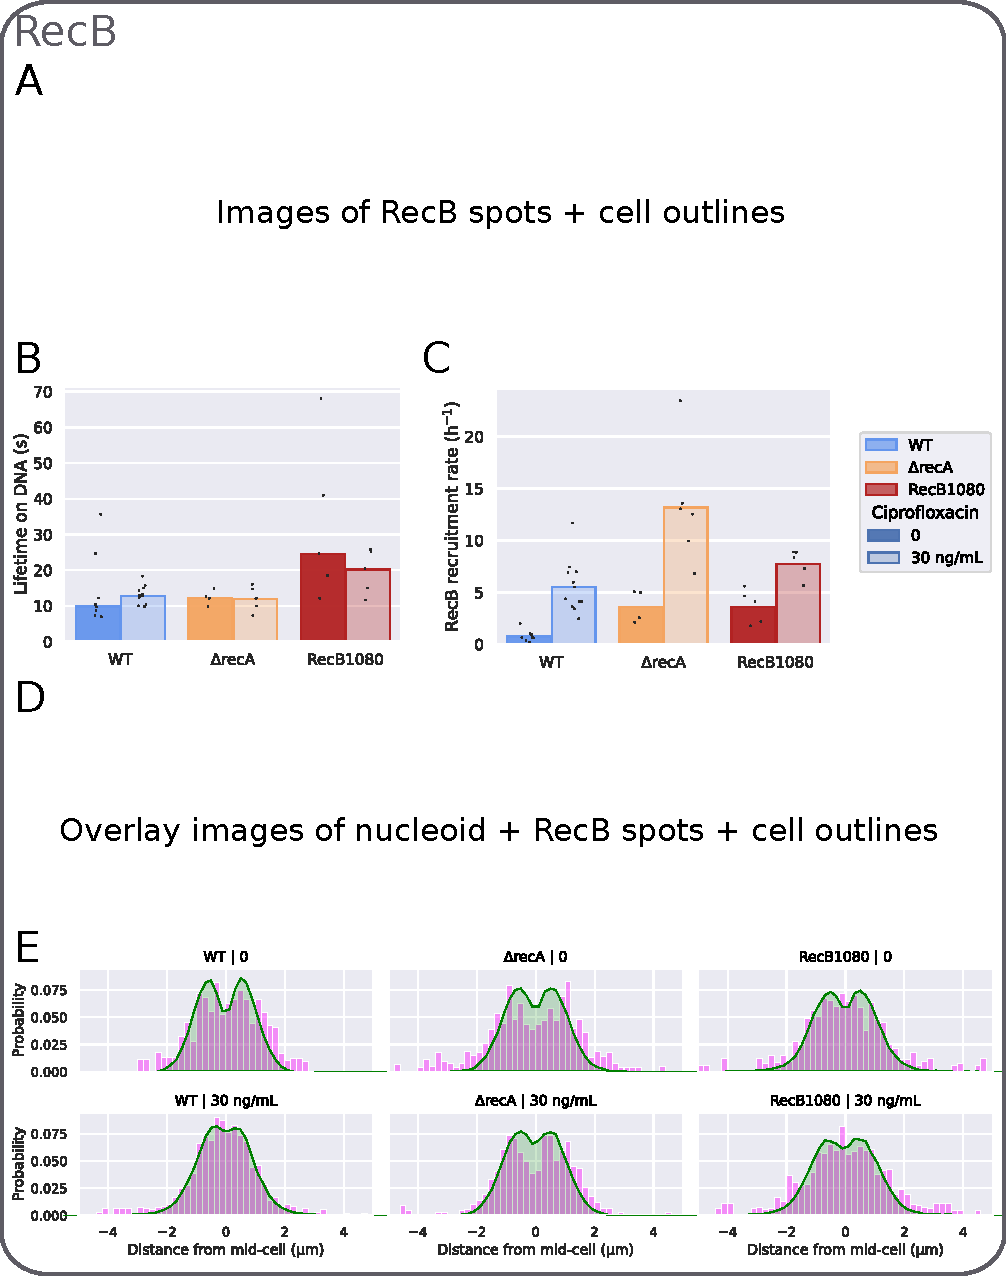
\includegraphics[width=\textwidth]{Fig5_mutants.pdf}
\end{center}
\caption{}
\label{Fig:mutants}
\end{figure*}

%% Unfortunately, mutant data are not well fitted by the bi-exponential model (why?). Therefore in this section we will rely on other metrics to quantify RecB binding to DNA.
To gain further insight into DSB repair by RecBCD, we imaged three different mutants in the repair pathway: a \textit{recA} deletion (\dreca), the RecB D$_{1080}$ $\rightarrow$ A (\teneighty) mutant, as well as the \dreca-\teneighty\ double-mutant. In the case of these mutants, fitting the RecB spot lifetime histogram with a bi-exponential decay model did not yield good results (Supp. Note \ref{note:mutants_fitting}). Therefore, we used a fixed, arbitrary lifetime threshold (12 seconds) to distinguish short- and long-lived RecB binding events.

%% There are more RecB spot per cell area in the mutants (Fig 5A). Because the level of DNA damage (endogenous or ciprofloxacin) is the same, we have to conclude that this represents slower dissociation of RecB from DNA.
%%% drecA has more RecB spots, both with and without cipro. This means that RecA plays a role in RecB dissociation from DNA, presumably associated with RecA loading
Compared to wild-type cells, all tested mutants showed a higher number of RecB spots per cell area (Figure \ref{Fig:mutants}A). Since the level of DNA damage (endogenous or 30 ng/mL ciprofloxacin) was the same for wild-type and mutant cells, this higher number of RecB spots must represent a slower dissociation of RecB from DNA. In light of this, the increased number of RecB spots in the \dreca\ mutant suggests that RecA plays a role in RecB dissociation from DNA, presumably associated with RecB's role in RecA loading.

%%% RecB1080 has even more spots than drecA. This means something else than RecA loading deficiency must make RecB dissociation difficult. We can hypothesise that it's RecB nuclease deficiency, which might make it hard for RecBCD to come off the DNA once it's threaded in
The \teneighty\ mutant is deficient in RecA loading, and nuclease activity.\cite{} It can bind DSBs and unwind the DNA duplex, but does not degrade the unwound strands. Even though it is unable to directly promote RecA loading, this still happens through an alternative pathway implicating RecJ and RecFOR.\cite{} Both in the presence and absence of ciprofloxacin, the \teneighty\ mutant shows more RecB spots than the WT or the \dreca\ mutant (\ref{Fig:mutants}A). This suggests that the increased lifetime of \teneighty\ on the DNA is not only due to its deficiency in RecA loading but also to the absence of its nuclease activity. Unwinding DNA without digesting it might make dissociation more challenging due to the DNA strands threading through the RecBCD complex.

%%% Entirely removing RecA in a 1080 background increases again the number of RecB spots per cell area, i.e. reduces the dissociation rate. This means in 1080 single-mutant, RecA still helps to dissociate RecB, presumably thanks to its loading by RecFOR.
Finally, the \dreca-\teneighty\ double-mutant displays a slight increase in the number of DNA-bound RecB per cell area compared to the \teneighty\ single-mutant (\ref{Fig:mutants}A). This means that in the \teneighty\ single-mutant, RecA still helps RecB to dissociate, presumably thanks to its loading by RecFOR.

%%%% START TO BE REMOVED %%%%
%% The proportion of long-lived spots (= "difficult" DNA repair, as determined in previous sections) increases either upon the addition of ciprofloxacin to WT cells, or when the dissociation process (RecA loading and/or RecB nuclease activity) is perturbed (Fig 5B).
In wild-type cells, we attributed the increase in long-lived RecB spots upon the addition of ciprofloxacin to an increase in the number of DSBs that are challenging to repair. In the absence of ciprofloxacin, mutant strains also display higher proportions of long-lived RecB spots (Figure \ref{Fig:mutants}B), matching with the interpretation that in these mutants, RecB stays bound to DNA for significantly longer times.

%%% There is no increase in the proportion of long-lived spots upon the addition of ciprofloxacin. This would indicate that the reason RecB stays bound longer under cipro resides in what happens between DSB recognition and RecA loading, NOT after RecA loading (e.g. duration of homology search).
Surprisingly, there was no increase in the proportion of long-lived spots in mutant strains upon the addition of ciprofloxacin. This suggests that the long-lived RecB spots created in the \dreca\ and \teneighty\ mutants are of a similar nature to those created by ciprofloxacin exposure in the wild-type (see Discussion).
%%%% END TO BE REMOVED %%%%

%% RecB spots in ΔrecA and/or 1080 background in the presence of ciprofloxacin are not centred as in WT.
%%% In ΔrecA there is no centring and even a slight "exclusion" of spots from the centre of the cell. This confirms the involvement of the SOS response in RecB spot centring.
Upon addition of high concentrations of ciprofloxacin (20-30 ng/mL), DNA-bound RecB molecules were mainly found in the centre of the cell (Figure \ref{Fig:high_cipro}A), which we attributed to SOS-dependent compaction of the bacterial chromosome. In the \dreca\ mutant at 30 ng/mL ciprofloxacin, DNA-bound RecB were found throughout the cell, with a slightly lower density towards the centre (Figure \ref{Fig:mutants}C). This pattern is similar to what would be expected of a DNA-bound protein in the absence of chromosome compaction (cite an Achilles article here?). This observation reinforces the idea that the centring of DNA-bound RecB observed in the wild-type under high ciprofloxacin depends on the SOS response.

%%% In 1080 there is no centring, but also no exclusion from the centre of the cell. This might correspond to a "mixed" population, where only a few spots get centred due to the delay in the SOS response
Interestingly, in the \teneighty\ mutant a more even distribution of DNA-bound RecB is observed. The density of bound molecules is not reduced at the centre of the cell, as was observed in the \dreca\ mutant (Figure \ref{Fig:mutants}C). This could be attributed to partial or delayed chromosome compaction, due to the largely reduced efficiency of RecA loading in the \teneighty\ mutant.

%%% In the double-mutant spots are again excluded from the cell centre, similarly to ΔrecA single mutant. This makes sense, as there will also be no SOS response in the double-mutant.
Finally, in the \dreca-\teneighty\ double-mutant, DNA-bound RecB molecules seem to adopt a similar phenotype to the \dreca\ single-mutant, where the density of molecules is reduced at the centre of the cell, consistent with a complete absence of SOS induction, and therefore no chromosome compaction.

